\documentclass[twoside]{article}
\usepackage{amsgen,amsmath,amstext,amsbsy,amsopn,amssymb,}
\usepackage{graphicx}
\usepackage{epsfig}

\setlength{\oddsidemargin}{0.1 in} \setlength{\evensidemargin}{-0.1
in} \setlength{\topmargin}{-0.6 in} \setlength{\textwidth}{6.5 in}
\setlength{\textheight}{10.5 in} \setlength{\headsep}{0.1 in}
\setlength{\parindent}{0 in} \setlength{\parskip}{0.1 in}

\newcommand{\homework}[2]{
   \pagestyle{myheadings}
   \thispagestyle{plain}
   \newpage
   \setcounter{page}{1}
   \noindent
   \begin{center}
   \framebox{
      \vbox{\vspace{2mm}
       \hbox to 6.28in { {\bf Math 4720:~Statistical Methods \hfill} }
       \vspace{6mm}
       \hbox to 6.28in { {\Large \hfill #1 (#2)  \hfill} }
       \vspace{6mm}
      \vspace{2mm}}
   }
   \end{center}
   \markboth{#1}{#1}
   \vspace*{4mm}
}

\newcommand{\bbF}{\mathbb{F}}
\newcommand{\bbX}{\mathbb{X}}
\newcommand{\bI}{\mathbf{I}}
\newcommand{\bX}{\mathbf{X}}
\newcommand{\bY}{\mathbf{Y}}
\newcommand{\bepsilon}{\boldsymbol{\epsilon}}
\newcommand{\balpha}{\boldsymbol{\alpha}}
\newcommand{\bbeta}{\boldsymbol{\beta}}
\newcommand{\0}{\mathbf{0}}

\begin{document}

\homework{$5^{th}$ and $6^{th}$ Week Summary}{2/20/25}

\begin{itemize}
\vspace{-.2in}
\item \textbf{Confidence intervals (Estimation)}
\subitem An interval calculated from the data, usually of the form: $\textrm{estimate} \pm \textrm{margin of error}$.
\subitem confidence interval for $\mu$ is $\bar{x} \pm z_{\alpha/2}\dfrac{\sigma}{\sqrt{n}}$ if
\subsubitem data is coming from normal population having unknown mean $\mu$ and known $\sigma$. or
\subsubitem large random sample from a non-normal population having unknown mean $\mu$ and known $\sigma$.
\item The confidence interval will have a specified \textbf{margin of error} $m$ when the sample size is: $n=\Bigl(\dfrac{z_{\alpha/2}\sigma}{m}\Bigr)^2$
\item \textbf{Hypothesis tests} (a.k.a., tests of significance) for \textit{population parameter}
\subitem $H_0$ is called the \textit{null hypothesis} while $H_a$ is called the \textit{alternative hypothesis}.
\subitem Usually the null hypothesis is a statement of \textit{no effect} or \textit{no difference}.
\subitem The claim about the population that we are \textit{trying to find evidence} for is the alternative hypothesis.
\subitem A \textbf{test statistic} calculated from the sample data measures how far the data diverge from the null hypothesis $H_0$. Define the test statistic $z=\dfrac{\bar{x}-\mu_0}{\sigma/\sqrt{n}}$
\subitem Decision Rule: Given fixed $\alpha=P(\textrm{Type-I Error})$.
\subsubitem $H_a: \mu > \mu_0$, Reject $H_0$ if $z>z_{\alpha}$
\subsubitem $H_a: \mu < \mu_0$, Reject $H_0$ if $z<-z_{\alpha}$
\subsubitem $H_a: \mu \neq \mu_0$, Reject $H_0$ if $|z|>-z_{\alpha/2}$
\item If we reject $H_0$ when in fact $H_0$ is true, this is a \textbf{Type I error}.
\subitem The significance level $\alpha$ of any fixed-level test is the probability of a Type I error.
\item If we fail to reject $H_0$ when in fact $H_a$ is true, this is a \textbf{Type II error}, also called $\beta$.
\subitem For one sided alternative test ($H_a:\mu>\mu_0$ or $H_a:\mu<\mu_0$ ): $\beta=P\Bigl(Z\leq z_\alpha-\dfrac{|\mu_0-\mu_a|}{\sigma/\sqrt{n}}\Bigr)$
\subitem For two sided alternative test ($H_a:\mu \neq \mu_0$): $\beta=P\Bigl(Z\leq z_{\alpha/2}-\dfrac{|\mu_0-\mu_a|}{\sigma/\sqrt{n}}\Bigr)$
\item The \textbf{power of a test against any alternative} is 1 minus the probability of a Type II error for that alternative: power $= 1 - \beta$.
\item \textbf{Power analysis} (Sample size determination):
\subitem For one sided alternative test ($H_a:\mu>\mu_0$ or $H_a:\mu<\mu_0$ ): $n=\sigma^2\dfrac{(z_\alpha+z_\beta)^2}{\Delta^2}$
\subitem For two sided alternative test ($H_a:\mu \neq \mu_0$): $n=\sigma^2\dfrac{(z_{\alpha/2}+z_\beta)^2}{\Delta^2}$
\end{itemize}

\begin{figure}[h]
\begin{center}
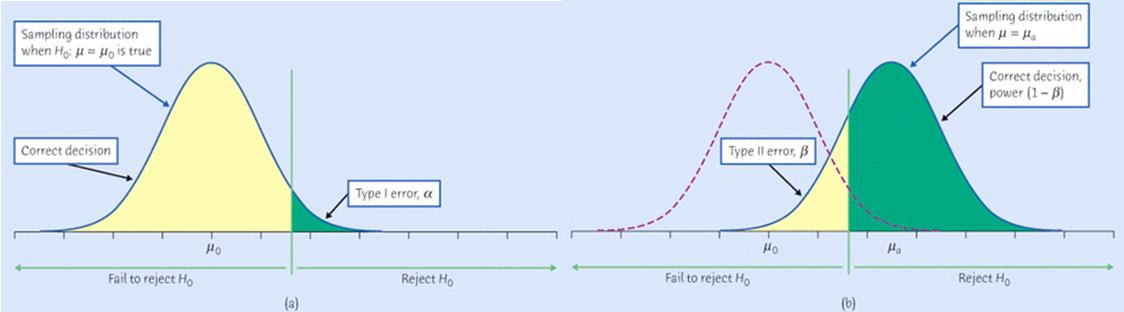
\includegraphics[angle=0, width=15.6 cm] {power.jpg}
\end{center}
\end{figure}
\end{document}


